\section{Симметричные протоколы}
\selectlanguage{russian}

Как отмечено ранее в разделе~\ref{section-protocols-classification} про классификацию протоколов, к симметричным будем относить те протоколы, которые используют примитивы только классической криптографии на секретных ключах. К ним относятся уже известные блочные шифры, криптографически стойкие генераторы псевдослучайных чисел (КСГПСЧ) и хеш-функции.

\subsection{Протокол Wide-Mouth Frog}\index{протокол!Wide-Mouth Frog|(}\label{section-protocols-wide-moth-frog}
Протокол Wide-Mouth Frog является, возможно, самым простым протоколом с доверенным центром. Его автором считается Майкл Бэрроуз (1989 год, \langen{Michael Burrows}, \cite{Burrows:Abadi:Needham:1990}). Протокол состоит из следующих проходов.

\begin{figure}
    \centering
    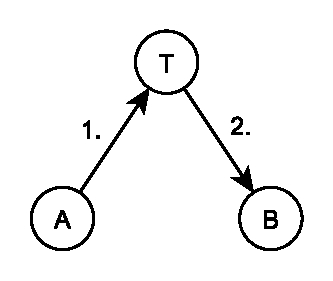
\includegraphics[width=0.5\textwidth]{pic/key_distribution-wide-mouth_frog}
    \caption{Схема взаимодействия абонентов и доверенного центра в протоколе Wide-Mouth Frog\label{fig:key_distribution-wide-mouth_frog}}
\end{figure}

\begin{protocol}
	\item[(1)] Алиса генерирует новый сеансовый ключ $K$
    \item[{}] $Alice \to \{ A, E_A \left( T_A, B, K \right) \} \to Trent$
	\item[(2)] $Trent \to \{ E_B \left( T_T, A, K \right) \} \to Bob$
\end{protocol}

По окончании протокола у Алисы и Боба есть общий сеансовый ключ $K$.

У данного протокола множество недостатков.

\begin{itemize}
	\item Генератором ключа является инициирующий абонент. Если предположить, что Боб -- это сервер, предоставляющий некоторый сервис, а Алиса -- это тонкий клиент, запрашивающий данный сервис, получается, что задача генерации надёжного сессионного ключа взваливается на плечи абонента с наименьшими мощностями.
	\item В протоколе общение с вызываемым абонентом происходит через доверенный центр. Как следствие, второй абонент может стать мишенью для DDOS-атаки с отражением (\langen{distributed denial-of-service attack}), когда злоумышленник будет посылать пакеты на доверенный центр, а тот формировать новые пакеты и посылать их абоненту. Если абонент подключён к нескольким сетям (с несколькими доверенными центрами), это позволит злоумышленнику вывести абонента из строя. Хотя защититься от подобной атаки достаточно просто, настроив соответствующим образом доверенный центр.
\end{itemize}

Однако самой серьёзной проблемой протокола является возможность применения следующих атак.

В 1995 году Рос Андерсон и Роджер Нидхем (\langen{Ross Anderson, Roger Needham}, \cite{Anderson:Needham:1995}) предложили вариант атаки на протокол, при котором злоумышленник (Ева) может бесконечно продлевать срок действия конкретного сеансового ключа. Идея атаки в том, что после окончания протокола злоумышленник будет посылать доверенному центру назад его же пакеты, дополняя их идентификаторами якобы инициирующего абонента.

\begin{protocol}
	\item[(1)] $Alice \to \{ A, E_A \left( T_A, B, K \right) \} \to Trent$
	\item[(2)] $Trent \to \{ E_B \left( T_T, A, K \right) \} \to Bob$
	\item[(3)] $Eva \to \{ B, E_B \left( T_A, A, K \right) \} \to Trent$
	\item[(4)] $Trent \to \{ E_A \left( T'_T, B, K \right) \} \to Alice$
	\item[(5)] $Eva \to \{ A, E_A \left( T'_T, B, K \right) \} \to Trent$
	\item[(6)] $Trent \to \{ E_B \left( T''_T, A, K \right) \} \to Bob$
	\item[{}] Повторять проходы 3 и 5, пока не пройдёт время, нужное для получения $K$.
\end{protocol}

С точки зрения доверенного центра, шаги 1, 3 и 5 являются корректными пакетами, инициирующими общение абонентов между собой. Метки времени в них корректны (если Ева будет успевать вовремя эти пакеты посылать). С точки зрения легальных абонентов каждый из пакетов является приглашением другого абонента начать общение. В результате произойдёт две вещи:

\begin{itemize}
	\item Каждый из абонентов будет уверен, что закончился протокол создания нового сеансового ключа, что второй абонент успешно аутентифицировал себя перед доверенным центром. И что для установления следующего сеанса связи будет использоваться новый (на самом деле -- старый) ключ $K$.
	\item После того, как пройдёт время, нужное злоумышленнику Еве для взлома сеансового ключа $K$, Ева сможет и читать всю переписку, проходящую между абонентами, и успешно выдавать себя за обоих из абонентов.
\end{itemize}

Вторая атака 1997 года Гэвина Лоу (\langen{Gavin Lowe}, \cite{Lowe:1997}) проще в реализации. В результате этой атаки Боб уверен, что Алиса аутентифицировала себя перед доверенным центром и хочет начать второй сеанс общения. Что, конечно, не является правдой, так как второй сеанс инициирован злоумышленником.

\begin{protocol}
	\item[(1)] $Alice \to \{ A, E_A \left( T_A, B, K \right) \} \to Trent$
	\item[(2)] $Trent \to \{ E_B \left( T_T, A, K \right) \} \to Bob$
	\item[(3)] $Eva \to \{ E_B \left( T_T, A, K \right) \} \to Bob$
\end{protocol}

В той же работе Лоу предложил модификацию протокола, вводящую явную взаимную аутентификацию абонентов с помощью случайной метки $R_B$ и проверки, что Алиса может расшифровать пакет с меткой, зашифрованной общим сеансовым ключом абонентов $K$. Однако данная модификация приводит к тому, что протокол теряет своё самое главное преимущество перед другими протоколами -- простоту.

\begin{protocol}
	\item[(1)] $Alice \to \{ A, E_A \left( T_A, B, K \right) \} \to Trent$
	\item[(2)] $Trent \to \{ E_B \left( T_T, A, K \right) \} \to Bob$
	\item[(3)] $Bob \to \{ E_K \left( R_B \right) \} \to Alice$
	\item[(4)] $Alice \to \{ E_K \left( R_B + 1 \right) \} \to Bob$
\end{protocol}

\index{протокол!Wide-Mouth Frog|)}


\subsection{Протокол Yahalom}\index{протокол!Yahalom|(}\label{section-protocols-yahalom}

Протокол Yahalom можно рассматривать как улучшенную версию протокола Wide-Mouth Frog\index{протокол!Wide-Mouth Frog} из раздела~\ref{section-protocols-wide-moth-frog}. Данный протокол <<перекладывает>> генерацию нового сессионного ключа на сторону доверенного центра, а также использует случайные числа для защиты от атак повтором.

\begin{figure}
	\centering
	\begin{sequencediagram}
		\newinst{Alice}{Alice}
		\newinst[3]{Trent}{Trent}
		\newinst[3]{Bob}{Bob}

		\mess{Alice}{$A$, $R_A$}{Bob}
		\mess{Bob}{$ B, E_B( A, R_A, R_B ) $}{Trent}
		\mess{Trent}{$ E_A( B, K, R_A, R_B )$, $E_B(A, K) $}{Alice}
		\mess{Alice}{$E_B( A, K )$, $E_K( R_B )$}{Bob}
	\end{sequencediagram}
	\caption{Диаграмма последовательности взаимодействия абонентов и доверенного центра в протоколе Yahalom\label{fig:key_distribution-yahalom}}
\end{figure}

\begin{protocol}
	\item[(1)] $Alice \to \{ A, R_A \} \to Bob$
	\item[(2)] $Bob \to \{ B, E_B( A, R_A, R_B ) \} \to Trent$
	\item[(3)] Трент генерирует новый сессионный ключ $K$
	\item[{}] $Trent \to \{ E_A( B, K, R_A, R_B ), E_B(A, K) \} \to Alice$
	\item[(4)] $Alice \to \{ E_B( A, K ), E_K( R_B ) \} \to Bob$
\end{protocol}

После того, как Боб провалидирует число $R_B$, присланное Алисой, стороны смогут использовать новый сессионный ключ $K$. Протокол, кроме генерации ключа, обеспечивает взаимную аутентификацию сторон:

\begin{itemize}
    \item Аутентификация Алисы перед Бобом происходит на 4-м проходе, когда Боб может провалидировать возможность Алисы зашифровать известное только ей (и Тренту) случайное число $R_B$ на ключе $K$.
    \item Аутентификация Боба перед Алисой происходит на 3-м проходе, когда Трент демонстрирует Алисе, что он получил случайное число $R_A$ именно от Боба.
\end{itemize}

Нужно отметить (\cite{Zhou:Yu:Pan:Wang:2016}), что в рамках протокола Боб никак не продемонстрировал, что он успешно получил новый сессионный ключ $K$ и может им оперировать (не выполнена цель G8). Сообщение от Алисы на 4-м проходе могло быть перехвачено или модифицировано злоумышленником. Но никакого ответа Алиса от Боба уже не ожидает и уверена, что протокол завершился успешно.

Также на 3-м проходе Трент не включает случайное число $R_B$ в сообщение $E_B(A, K)$, что позволяет Алисе, действуя не из лучших побуждений, заставить Боба принять старый сессионный ключ (рис.~\ref{fig:key_distribution-yahalom-attack}).

\begin{figure}
	\centering
	\begin{sequencediagram}
		\newinst{Alice}{Alice}
		\newinst[3]{Trent}{Trent}
		\newinst[3]{Bob}{Bob}

		\mess{Alice}{$A$, $R_{A2}$}{Bob}
		\mess{Bob}{$ B, E_B( A, R_{A2}, R_{B2} ) $}{Trent}
		\mess{Trent}{$ E_A( B, K_2, R_{A2}, R_{B2} )$, $E_B(A, K_2) $}{Alice}
		\mess{Alice}{$E_B( A, K_1 )$, $E_{K_1}( R_{B2} )$}{Bob}
	\end{sequencediagram}
	\caption{Диаграмма последовательности атаки на протокол Yahalom для использованием старого сессионного ключа\label{fig:key_distribution-yahalom-attack}}
\end{figure}

\begin{protocol}
	\item[(1)] $Alice \to \{ A, R_A \} \to Bob$
	\item[(2)] $Bob \to \{ B, E_B( A, R_A, R_B ) \} \to Trent$
	\item[(3)] Трент генерирует новый сессионный ключ $K_2$
	\item[{}] $Trent \to \{ E_A( B, K, R_A, R_B ), E_B(A, K_2) \} \to Alice$
	\item[(4)] Алиса использует старый сессионный ключ $K_1$ и сообщение $E_B( A, K_1 )$ из старого сеанса протокола
	\item[{}] $Alice \to \{ E_B( A, K_1 ), E_{K_2}( R_B ) \} \to Bob$
\end{protocol}

Протокол Yahalom послужил основной большому количеству научных работ, связанных с автоматизированным анализом стойкости криптографических протоколов и имел несколько <<улучшенных>> вариантов. Однако о широком использовании данного протокола в реальных информационных системах неизвестно.

\index{протокол!Yahalom|)}


\subsection{Протокол Нидхема~---~Шрёдера}\index{протокол!Нидхема~---~Шрёдера|(}\label{section-protocols-needham-schroeder}
\selectlanguage{russian}

Протокол Нидхема~---~Шрёдера (\langen{Roger Needham, Michael Shroeder}, 1979,~\cite{Needham:Schroeder:1978}) похож на модифицированный протокол Wide-Mouth Frog, но отличается тем, что доверенный центр (Трент) во время работы основной части протокола не общается со вторым абонентом. Первый абонент получает от доверенного центра специальный пакет, который он без всякой модификации отправляет второму абоненту.

\begin{figure}
    \centering
    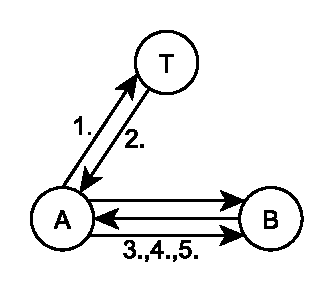
\includegraphics[width=0.5\textwidth]{pic/key_distribution-needham-schroeder}
    \caption{Схема взаимодействия абонентов и доверенного центра в протоколе Нидхема~---~Шрёдера\label{fig:key_distribution-needham-schroeder}}
\end{figure}

\begin{samepage}\begin{itemize}
	\item[(1)] $ Alice	\to \{ A, B, R_A \}						\to Trent $
	\item[(2)] $ Trent	\to \{ E_A \left( R_A, B, K, E_B \left( K, A \right) \right) \}	\to Alice $
	\item[(3)] $ Alice	\to \{ E_B \left( K, A \right) \}				\to Bob $
	\item[(4)] $ Bob	\to \{ E_K \left( R_B \right) \}				\to Alice $
	\item[(5)] $ Alice	\to \{ E_K \left( R_B - 1 \right) \}				\to Bob $
\end{itemize}\end{samepage}

Протокол удобен с точки зрения сетевого взаимодействия участников (рис.~\ref{fig:key_distribution-needham-schroeder}). И общение с доверенным центром, и с конечным участником (Бобом) начинается только по инициативе первого участника (Алисы). При возникновении любых проблем передачи пакетов их видит именно то лицо, которое заинтересованно в получении ключей и доступов\footnote{Сравните с протоколом Yahalom, в котором при возникновении проблемы общения Трента и Алисы на третьем проходе Тренту потребовалось бы уведомить об этом Боба, а Бобу, в свою очередь, Алису.}. И если бы общение шло с использование протокола TCP/IP, потребовалось бы всего 2 сессии протокола TCP для выработки ключа. Причём последнюю сессию можно не закрывать, а использовать как сессию для дальнейшего взаимодействия уже с ключом $K$.

Протокол обеспечивает и двустороннюю аутентификацию сторон, и, казалось бы, защиту от атак с повторной передачей (\langen{replay attack}). Последнее делается с помощью введения уже известных по модифицированному протоколу Wide-Mouth Frog случайных меток $R_A$ и $R_B$. Действительно, без знания ключа злоумышленник не сможет выдать себя за Алису перед Бобом (так как не сможет расшифровать пакет с зашифрованной меткой $R_B$).

Однако протокол уязвим к атаке с известным сеансовым ключом. Если злоумышленник сумеет в какой-то момент времени получить ранее использованный сессионный ключ $K$, он сможет убедить Боба, что он является Алисой, и что это новый сессионный ключ. Для этого ему понадобится переданный ранее по открытому каналу пакет из пункта 3 протокола.

\begin{itemize}
	\item[(1)] $ Eva \to \{ A, B, R_A \} \to Trent $
	\item[(2)] $ Trent \to \{ E_A \left( R_A, B, K, E_B \left( K, A \right) \right) \}	\to Alice $
	\item[(3)] $ Alice \to \{ E_B \left( K, A \right) \} \to Bob $
	\item[(4)] $ Bob \to \{ E_K \left( R_B \right) \} \to Alice $
	\item[(5)] $ Alice \to \{ E_K \left( R_B - 1 \right) \} \to Bob $
	\item[{}]  $\dots$ по прошествии некоторого времени $\dots$
	\item[(6)] $ Eva~(Alice) \to \{ E_B \left( K, A \right) \} \to Bob $
	\item[(7)] $ Bob \to \{ E_K \left( R_B \right) \} \to Eva~(Alice) $
	\item[(8)] $ Eva (Alice) \to \{ E_K \left( R_B - 1 \right) \} \to Bob $
\end{itemize}

Относительно мелкий недостаток протокола состоит ещё и в том, что во втором пакете доверенный центр в зашифрованном виде передаёт то, что в третьем шаге пересылается по открытому каналу ($E_B \left( K, A \right)$).

Если в протокол добавить метки времени, тем самым ограничив время возможного использования сессионного ключа, а также исправить мелкий недостаток с двойным шифрованием, можно получить протокол, который лежит в основе распространённого средства аутентификации <<Kerberos>> для локальных сетей.

\index{протокол!Нидхема~---~Шрёдера|)}


\section{Система Kerberos для локальной сети}
\selectlanguage{russian}

Система аутентификации и распределения ключей Kerberos основана на протоколе Нидхэма--Шредера. Самые известные реализации протокола Kerberos включают Microsoft Active Directory и ПО Kerberos с открытым кодом для Unix.

Протокол предназначен для решения задачи аутентификации и распределения ключей в рамках локальной сети, в которой есть группа пользователей, имеющих доступ к набору сервисов, и требуется обеспечить единую аутентификацию для всех сервисов. Протокол Kerberos сделан полностью на симметричных криптосистемах. Секретный ключ используется для взаимной аутентификации.

Естественно, что в нелокальной сети интернет невозможно секретно создать и распределить пары секретных ключей и поэтому Kerberos построен для (виртуальной) локальной сети.

В протоколе используется 4 типа субъектов:

\begin{itemize}
    \item пользователи системы $C_i$,
    \item сервисы $S_i$, доступ к которым имеют пользователи,
    \item сервер аутентификации AS (authentication server), который производит аутентификацию пользователей по паролям и/или смарт-картам только один раз и выдает секретные сеансовые ключи для дальнейшей аутентификации,
    \item сервер выдачи мандатов TGS (ticket granting server) для аутентификации доступа к запрашиваемым сервисам; аутентификация выполняется по сеансовым ключам\index{ключ!сеансовый}, выданным сервером AS.
\end{itemize}

Для работы протокола требуется заранее распределить следующие секретные симметричные ключи для взаимной аутентификации.
\begin{itemize}
    \item Ключи $K_{C_i}$ между пользователем $i$ и сервером AS. Как правило, ключом служит обычный пароль\index{пароль}, точнее результат хэширования пароля. Может быть использована и смарт-карта.
    \item Ключ $K_{TGS}$ между серверами AS и TGS.
    \item Ключи $K_{S_i}$ между сервисами $S_i$ и сервером TGS.
\end{itemize}

\begin{figure}[h!]
	\centering
	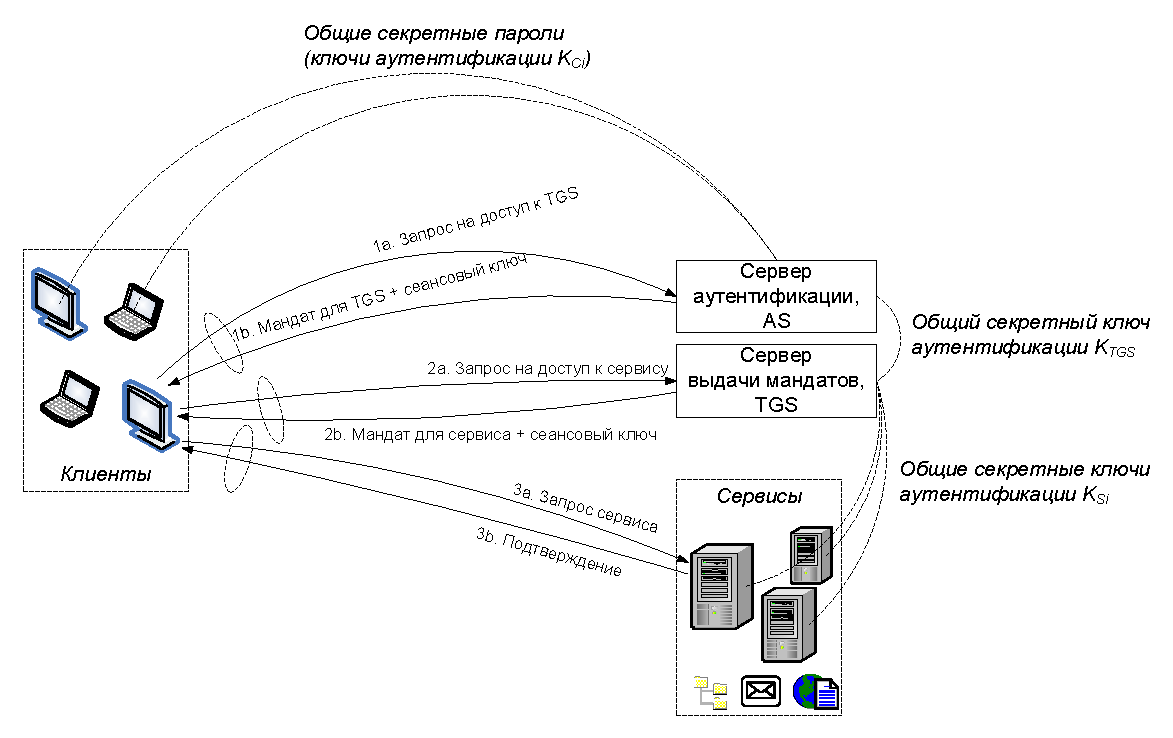
\includegraphics[width=\textwidth]{pic/kerberos}
	\caption{Схема аутентификации и распределения ключей Kerberos\label{fig:kerberos}}
\end{figure}

На рис. \ref{fig:kerberos} представлена схема протокола, состоящая из 6 шагов.

Введем обозначения для протокола между пользователем $C$ с ключом $K_C$ и сервисом $S$ с ключом $K_S$.
\begin{itemize}
    \item $ID_C, ID_{TGS}, ID_S$ -- идентификаторы пользователя, сервера TGS и сервиса $S$, соответственно,
    \item $t_i, \tilde{t}_i$ -- запрашиваемые и выданные границы времени действия сеансовых ключей аутентификации,
    \item $ts_i$ -- метка текущего времени (timestamp),
    \item $N_i$ -- одноразовая метка (nonce)\index{одноразовая метка}, псевдослучайное число, для защиты от атак воспроизведения сообщений,
    \item $K_{C,TGS}, K_{C,S}$ -- выданные сеансовые ключи аутентификации пользователя и сервера TGS, пользователя и сервиса $S$, соответственно,
    \item $T_{TGS} = E_{K_{TGS}}(K_{C,TGS} ~\|~ ID_C ~\|~ \tilde{t}_1)$ -- мандат (ticket) для TGS, который пользователь расшифровать не может.
    \item $T_{S} = E_{K_S}(K_{C,S} ~\|~ ID_C ~\|~ \tilde{t}_2)$ -- мандат для сервиса $S$, который пользователь расшифровать не может.
    \item $K_1, K_2$ -- обмен информацией для генерирования общего секретного симметричного ключа дальнейшей коммуникации, например, по протоколу Диффи--Хеллмана.
\end{itemize}

Схема протокола следующая.
\begin{enumerate}
    \item Первичная аутентификация пользователя по паролю, получение сеансового ключа $K_{C,TGS}$ для дальнейшей аутентификации. Это действие выполняется один раз для каждого пользователя, чтобы уменьшить риск компроментации пароля.
        \begin{enumerate}
            \item $C \rightarrow AS: ~~ ID_C ~\|~ ID_{TGS} ~\|~ t_1 ~\|~ N_1$.
            \item $C \leftarrow AS: ~~ ID_C ~\|~ T_{TGS} ~\|~ E_{K_C}( K_{C,TGS} ~\|~ \tilde{t}_1 ~\|~ N_1 ~\|~ ID_{TGS})$.
        \end{enumerate}
    \item Аутентификация сеансовым ключом $K_{C,TGS}$ на сервере TGS для запроса доступа к сервису выполняется один раз для каждого сервиса. Получение другого сеансового ключа аутентификации $K_{C,S}$.
        \begin{enumerate}
            \item $C \rightarrow TGS: ~~ ID_S ~\|~ t_2 ~\|~ N_2 ~\|~ T_{TGS} ~\|~ E_{K_{C,TGS}}(ID_C ~\|~ ts_1)$.
            \item $C \leftarrow TGS: ~~ ID_C ~\|~ T_{S} ~\|~ E_{K_{C,TGS}}( K_{C,S} ~\|~ \tilde{t}_2 ~\|~ N_2 ~\|~ ID_S)$.
        \end{enumerate}
    \item Аутентификация сеансовым ключом $K_{C,S}$ на сервисе $S$ -- создание общего сеансового ключа дальнейшего взаимодействия.
        \begin{enumerate}
            \item $C \rightarrow S: ~~ T_{S} ~\|~ E_{K_{C,S}}(ID_C ~\|~ ts_2 ~\|~ K_1)$.
            \item $C \leftarrow S: ~~ E_{K_{C,S}}( ts_2 ~\|~ K_2)$.
        \end{enumerate}
\end{enumerate}

Аутентификация и проверка целостности достигается сравнением идентификаторов, одноразовых меток и меток времени внутри зашифрованных сообщений после расшифрования с их действительными значениями.

Некоторым недостатком схемы является необходимость синхронизации часов между субъектами сети.

